$if(has-frontmatter)$
  \frontmatter
$endif$
  
  $if(title)$
  \maketitle
$endif$

\pagenumbering{roman}

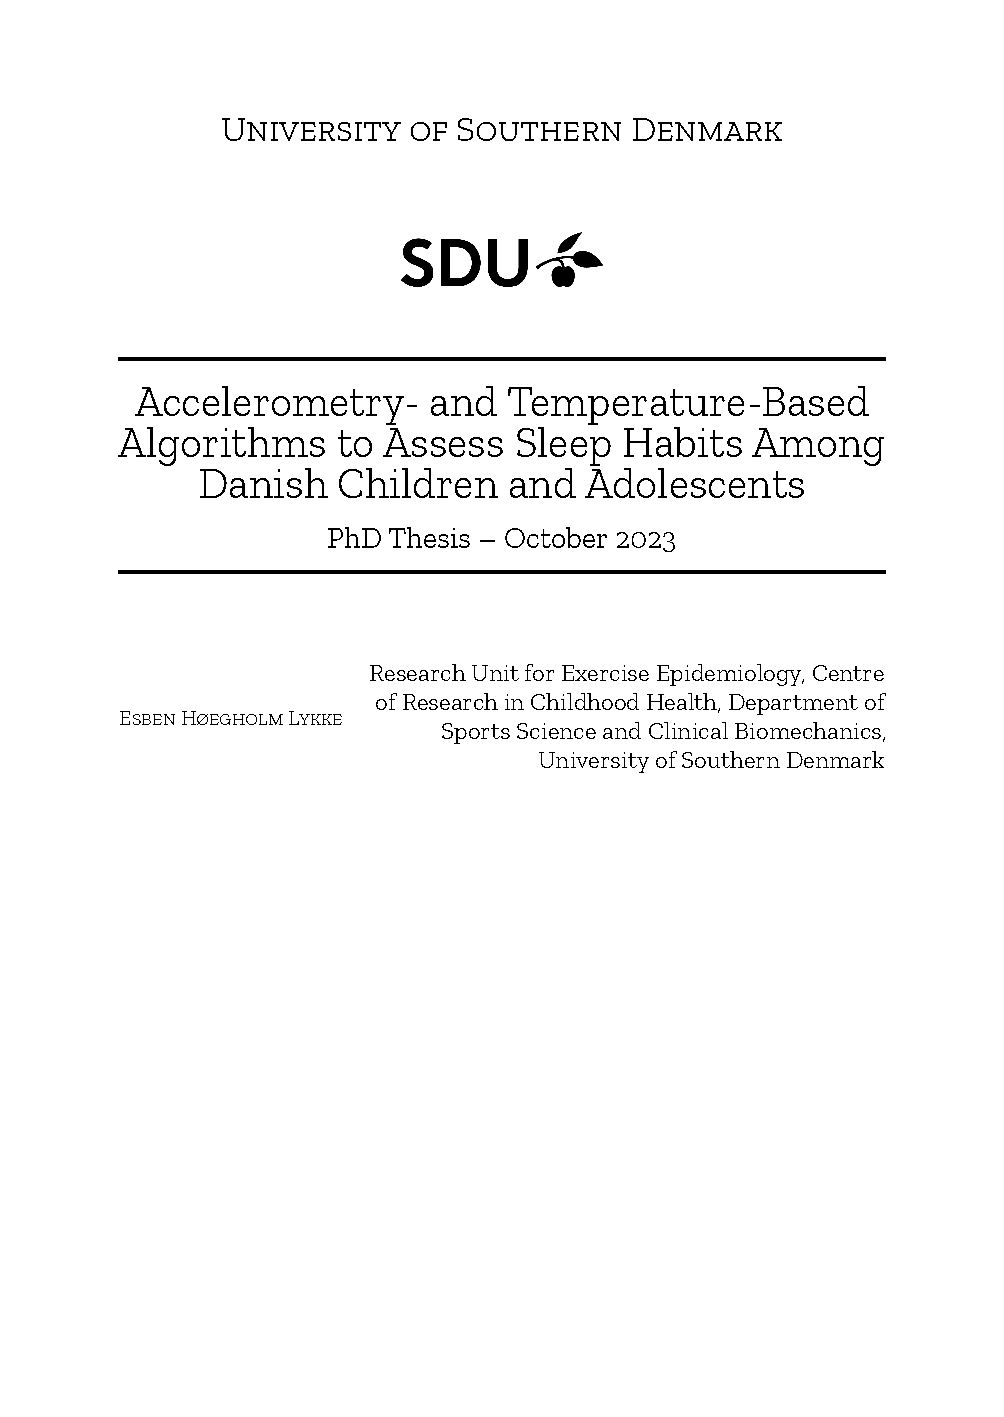
\includepdf[pages=-]{titlepage.pdf}

\newpage

\textsf{\textbf{\Large{Supervisor}}}

\vspace*{\baselineskip}

Associate Professor Jan Christian Brønd, PhD

Research Unit for Exercise Epedimiology, Centre of Research in Childhood Health, Department of Sports Science and Clinical Biomechanics, University of Southern Denmark, Odense, Denmark

\vspace{2cm}

\textsf{\textbf{\Large{Assessment Committee}}}

\vspace*{\baselineskip}

\textbf{Chair}

Professor WSR Jasper Schiperijn, PhD

Research Unit of Active Living, Danish centre for motivation and behaviour science, Playground Research, Department of Sports Science and Clinical Biomechanics, University of Southern Denmark, 5230 Odense, Denmark

\textbf{Opponents}

Associate Professor Samuel Emil Schmidt, PhD

Department of Health Science and Technology, Aalborg University, Denmark

Associate Professor Alex Rowlands, PhD

Diabetes Research Centre, NIHR Leicester Biomedical Research Centre - Lifestyle Theme, University of Leicester, United Kingdom

\vspace{2cm}

\textsf{\textbf{\Large{Funding}}}

\vspace*{\baselineskip}

The research presented in this thesis was generously funded by TrygFonden, under grant numbers ID 130081 and 115606, and by the European Research Council, under grant number 716657. Additional support was provided by a one-year scholarship from the Faculty of Health Sciences.

\newpage

%----------------------------------------------
  %   Preface
%----------------------------------------------
  
\textsf{\textbf{\Large{Preface}}}

\vspace*{\baselineskip}

The journey of my PhD has been a fulfilling expedition, layered with explorations, discoveries, struggles, and growth. This endeavor was fueled by my interest in understanding the objective measurements of physical behavior and sleep. During my Masters, I found myself increasingly engrossed in these domains.

My subsequent role as a research assistant at Aarhus University opened another dimension of learning for me. The works of my peers, employing machine learning and advanced statistics on accelerometer data, intrigued me. It was as if I found the nexus of my research interests, a perfect alignment that seamlessly fused my curiosities and passions.

One of the most significant hurdles was my limited experience with programming and machine learning, which proved to be a steep learning curve. However, through persistence, I slowly developed the necessary skills to analyze and interpret my data effectively. Another major setback was the failed data collection for my third paper. I spent months visiting families, mounting an ambulatory PSG device on children before bedtime, and facing the harsh reality of dealing with poor data quality.

This thesis brings together my explorations and findings across three papers that carry a consistent emphasis on improving and validating methods to leverage accelerometer data for studying human behaviors. The common thread across these papers is the application of innovative methods, particularly machine learning techniques, to enhance the utility, reliability, and accuracy of free-living accelerometer data for monitoring human sleep and physical activity. The work presented here constitutes a substantial contribution to the field of sleep and physical activity research, particularly in the context of large-scale studies.

Two of these papers have already found their place in peer-reviewed scientific journals, and the third is under review. All of these works are included as appendices to this thesis, and their content has been weaved into the fabric of this thesis.

As I look back at my journey through the PhD program, I am grateful for this opportunity to delve deep into a subject that I am passionate about and to contribute to a field that is evolving rapidly. This experience has instilled in me a sense of tenacity and patience, qualities that I have come to value deeply. I learned that even the most frustrating problems have solutions, and the path to those solutions often leads to personal growth and novel insights.

As I stand on the precipice of my future, I am filled with a sense of anticipation and excitement for the possibilities that lie ahead. I am eager to explore new horizons, to encounter new challenges, and to continue growing as a researcher and as an individual. However, wherever I go and whatever I do, I will carry with me the memories, experiences, and lessons from this incredible journey.

These years have shaped me in ways I could never have imagined at the outset, and for that, I am profoundly grateful. As I close this chapter of my life, I do so with a sense of accomplishment and a promise of continued exploration and discovery in my field. After all, every ending is but a new beginning, and I look forward to the adventures that await.

\newpage

%----------------------------------------------
  %   Acknowledgement
%----------------------------------------------
  
\textsf{\textbf{\Large{Acknowledgment}}}

\vspace*{\baselineskip}

Throughout this journey, there have been several people who have influenced, inspired, and supported me. My Main Supervisor, Jan Christian Brønd, deserves special mention for his guidance and patience. His commitment to nurturing my development as a researcher and lecturer has been instrumental. Our collaborative dialogues, be it at the office or during examinations, have been pivotal in my growth. I also extend my sincere gratitude to my co-supervisors [insert name 2] and [insert name 3], and my colleague [insert name 4], who have always provided invaluable insights and perspectives.

Amidst all the academic pursuits, my family remained the cornerstone of my journey. My wife, the bedrock of our family, kept our home running smoothly and offered endless support and curiosity about my work. The joy and love from my four children were my constant sources of motivation and inspiration.

The PhD journey has taught me the importance of rigour and attention to detail. My approach to work has been permanently shaped by my experience as a researcher. The discipline and precision that is required in research has translated into my everyday life, impacting my approach to problem-solving, decision-making, and even communication. It's impressive how research is not merely a vocation but a lens through which we view the world.

There were also moments of immense joy and satisfaction, like finally solving a complex analytical problem, having my work accepted for publication, or simply receiving positive feedback from a student or a colleague. Those moments fueled my motivation and reminded me of the importance and impact of my work.

One of the most rewarding aspects of this journey was the opportunity to be part of an international recognized and experienced research group. This gave me the chance to work with and learn from some of the most talented people in my field, to discuss ideas and collaborate on projects, and to be part of a collective effort to advance knowledge and understanding in our field.

In retrospect, this PhD journey has been much more than a professional pursuit. It has been a personal voyage of self-discovery and growth. Through the highs and lows, the victories and setbacks, the late nights and early mornings, I've discovered a resilience in myself that I hadn't known before. I found that I could rise to challenges, learn from failures, and continue to strive for excellence, no matter the odds.

In closing, I wish to express my deep gratitude for all those who have supported me throughout this journey - my supervisors, colleagues, friends, and family. Their faith in my abilities and their constant encouragement have been my pillars of strength. I hope that the work presented in this thesis reflects the depth of my dedication and the extent of my learning journey.

\newpage

\textsf{\textbf{\Large{Included Papers}}}

\vspace{2cm}

\begin{center}

Paper I

\textsf{Manual Annotation of Time in Bed Using Free-Living Recordings of Accelerometry Data}

published in \href{https://doi.org/10.3390/s21248442}{Sensors}

\vspace{2cm}
Paper II

\textsf{Generalizability and Performance of Methods to Detect Non‑Wear with Free‑Living Accelerometer Recordings}

published in \href{https://doi.org/10.1038/s41598-023-29666-x}{Scientific Reports}

\vspace{2cm}
Paper III 

\textsf{Improving Sleep Quality Estimation: A Comparative Study of Machine Learning and Deep Learning Techniques Utilizing Free-Living Accelerometer Data from Thigh-Worn Devices and EEG-Based Sleep Tracking}

Submitted to \href{https://www.nature.com/npjdigitalmed/}{npj Digital Medicine}

\end{center}

\newpage